\chapter{Números mágicos}
\label{c2}

O objetivo deste capítulo é apresentar

\section{Clusters}
\label{c2-clusters}

\textit{Clusters} são agregados de átomos ou moléculas, que variam desde dois à vários milhares de átomos, encontram-se na fronteira entre os átomos e o \textit{bulk}\footnote{\textit{Entende-se como "bulk" um conjunto de partículas sólidas grande o suficiente para que a média estatística de suas propriedades seja independente do número de partículas\cite{bulk}}}\cite{Heer,Brack}. 

No geral, os \textit{clusters} atômicos são classificados de acordo com seu tamanho: pequenos, médios ou grandes. Aglomerados classificados como pequenos, apresentam propriedades quânticas que possuem uma grande dependência com número de partículas e não variam suavemente com seu tamanho, diferentemente dos \textit{clusters} médios e grandes. Normalmente os \textit{clusters} são ditos pequenos, quando contém mais do que algumas centenas ou quase mil partículas, os nano-agregados considerados grandes possuem muitas milhares de partículas e suas propriedades tendem a seguir a tendência das propriedades da matéria um \textit{bulk} \cite{livro_cluster}.

A análise da distribuição do tamanho dos \textit{clusters}, advindos dos espectros
de massa, pode prover critérios fundamentais para as tendências estruturais e energéticas \cite{dissertacao_anderson}, no qual está focado este trabalho.

Buscando entender melhor essas transições bruscas de propriedades, segundo Bernd v. Issendorff (2009), podemos começar os estudos pensando em uma descrição simples, porém suficiente, do modo como se comportam os elétrons de um metal. Assumindo um sistema de elétrons livres isso implica que os elétrons da camada de valência se movem através da rede de metal infinita agindo como partículas livres. Assim, as funções de onda eletrônicas são apenas ondas planas tornando qualquer comprimento de onda possível. Uma mudança significativa ocorre quando o metal possuí dimensões nanoscópicas ou são nanopartículas. Agora, as funções de onda formam ondas estacionárias entre as superfícies da partícula, o que é possível somente para certos comprimentos de onda. Uma consequência direta é a discretização da densidade eletrônica de estados: a banda de valência contínua se divide em um número infinito de estados. Este é o chamado efeito de tamanho quântico, que pode levar a mudanças significativas propriedades das partículas de metal. Pode-se esperar que tais efeitos possam ser mais claramente vistos para um metal que se aproxime do comportamento ideal dos elétrons livres \cite{capitulo_livro_shell}. A Figura \ref{fig:transicao_cluster_solido} mostra a mudança das propriedades de um material enquanto \textit{clusters} e enquanto sólido, ilustrando o que foi dito.


\begin{figure}
  \centering
  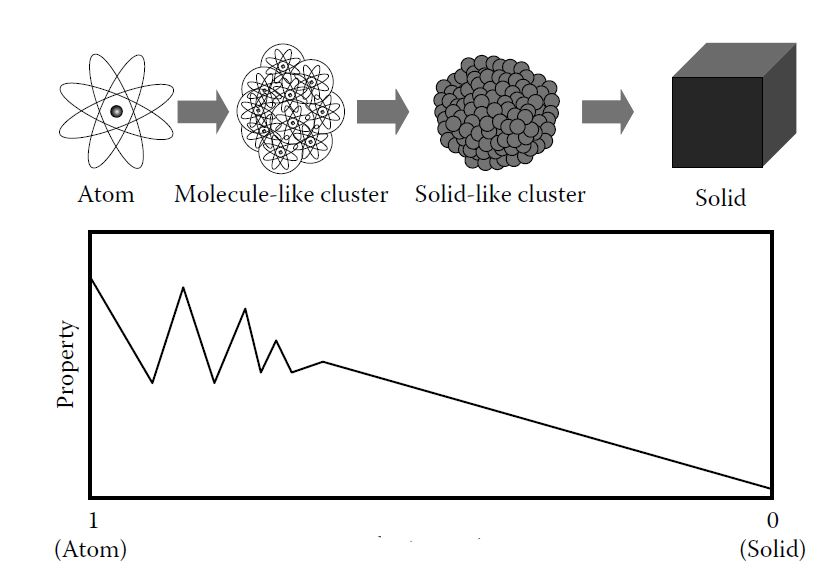
\includegraphics[width=0.8\textwidth]{images/clusters/atomo_cluste_solido}
  \caption{Esquema de transformação dimensional de átomos através de pequenos e grandes \textit{clusters} para o estado sólido. Quando os \textit{clusters} são pequenos cada átomo adicionado é importante, por isso as propriedades mudam
de forma abruptamente com o tamanho. Quando os \textit{clusters} se tornam grandes,
propriedades mudam suavemente\cite{cap06_Nanophysics}. Adaptado.  }
  \label{fig:transicao_cluster_solido}
\end{figure}

Uma das mudanças de propriedades interessantes é o surgimento de características semicondutoras em nanopartículas metálicas, que pode ser vista de Figura\ref{fig:carac_metal}.


\begin{figure}
  \centering
  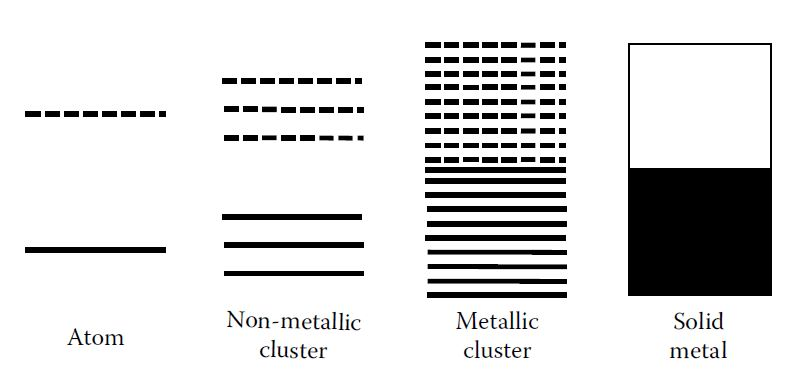
\includegraphics[width=0.7\textwidth]{images/clusters/carac_metal}
  \caption{ Esquema de transformação estrutural de energia a partir de átomos de metal através de pequenos e grandes \textit{clusters} para o metal sólido. Abaixo de um certo tamanho de \textit{clusters}, no qual as bandas vazia e povoada se fundem, um \textit{clusters} de átomos de metal pode ter uma estrutura de energia semelhante a um semicondutor.\cite{dissertacao_anderson}  }
  \label{fig:carac_metal}
\end{figure}



À medida que o número de átomos aumenta, também aumenta o número de níveis de energia disponíveis, até que a divisão entre níveis ocupados e desocupados se torna menor do que a energia térmica, momento em que o cluster começa a exibir comportamento metálico. Para os tamanhos maiores que esse tamanho crítico de transição, os aglomerados metálicos se comportarão como pequenos pedaços do metal macroscópico correspondente., mas com uma alta relação superfície / volume dependente do tamanho, como discutido em conexão com a Figura 7.2 [4]. Abaixo desse tamanho crítico, os clusters de elementos metálicos podem ter propriedades semelhantes a semicondutores.


Deixando de lado os casos limites, que geram ambiguidades a diferença entre \textit{cluster} e moléculas, encontra-se no fato que estas, no geral, possuem composições específicas e bem definidas e, na grande maioria dos casos, suas estruturas também são bem definidas, tendo  assim um número restrito de átomos; diferente um \textit{cluster}, como exemplo podemos citar um \textit{cluster} de prata que pode conter de 2, 15, 100, ou qualquer outro número de átomos de prata respeitando os limites impostos para um \textit{cluster}. Esses por sua vez também não possuem uma estrutura única, como podemos ver na Figura \ref{fig:estrutura_cluster_ag}, e para sua maioria, à medida que o número de partículas do \textit{cluster} aumenta, o número de estruturas estáveis disponíveis torna-se mais abundante. 

\begin{figure}
  \centering
  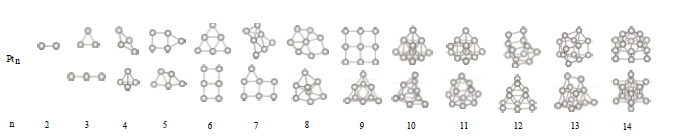
\includegraphics[width=1\textwidth]{images/clusters/estrutura_cluster_ag}
  \caption{ Exemplo de estruturas de \textit{clusters} de prata.\cite{dissertacao_anderson}  }
  \label{fig:estrutura_cluster_ag}
\end{figure}






O histórico de estudo da organização espacial dos arranjos atômicos cristalinos frutificaram na premiação de um Nobel em 1915, para William Henry Bragg e William Lawrence Bragg, nota-se então a complexidade desse tipo de pesquisa. A análise das estruturas dos \textit{clusters} é fundamental para compreender suas propriedades e  dispor de seus potenciais tecnológicos, isso também torna-se muito importante para o domínio da estabilidade das nanopartículas. 



Em 1984, Knight et al \cite{electronic_Shell_sodium}, realizou um experimento com nanopartículas de sódio (Na), com N átomos por conglomerado (N = 4-100), e foram encontrado padrões, com picos bem definidos, no espectro de massa de \textit{clusters} de Na em fase gasosa, podendo ser visto na Figura \ref{fig:espec_na}(a). Cada pico do espectro representa o número de 
aglomerados de um determinado N detectado. Note a presença de picos maiores, quando comparado com os outros picos, para certas massas correspondentes à N = $8, 20, 40, 58$ e $92$, onde podemos notar padrões. Os \textit{clusters} mais abundantes
no espectro de massa são considerados relativamente mais estável. Podemos destacar a estrutura eletrônica dessas nanopartículas como a causa de maior estabilidade. Esses picos foram apelidados de \textit{clusters mágicos} ou \textit{clusters com números mágicos de átomos}.




\begin{figure}
  \centering
  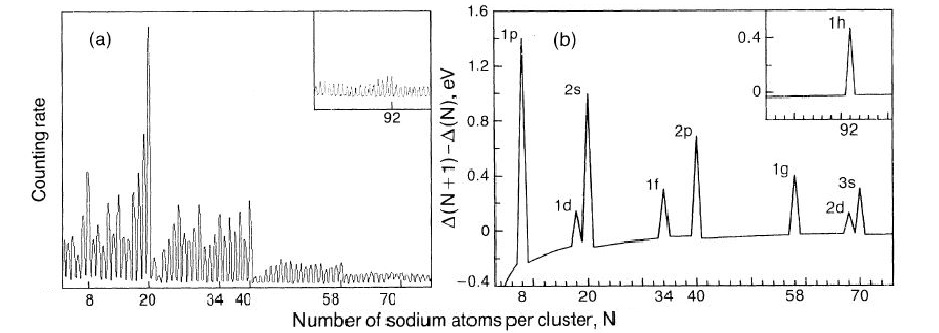
\includegraphics[width=1\textwidth]{images/clusters/NA_knight}
  \caption{(a) Espectro de massa de \textit{clusters} de sódio, N = 4-75.
  (b) A mudança calculada na diferença de energia eletrônica. Os picos protuberantes correspondem aos orbitais de casca fechada.\cite{electronic_Shell_sodium}  }
  \label{fig:espec_na}
\end{figure}


Podemos explicar a ocorrência desses \textit{clusters mágicos} foi suposto o efeitos de preenchimento de camadas eletrônicas, em que a combinação entre o espectro de estados
quantizados e o princípio de exclusão de Pauli resulta em efeitos de camada \cite{Brack}.O modelo quântico de \textit{Jellium} \cite{Heer}, foi usado com sucesso para explicar a ocorrência desses \textit{clusters mágicos} \cite{capitulo_livro_shell}.

As características dos espectros de massa de outros metais alcalinos e também dos metais nobres, seguem um padrão semelhante ao do sódio. Para as nanopartículas consideradas grandes, o padrão de números mágicos aparece diferente, e no geral ele é atribuído como uma consequência do preenchimento de camadas geométricas ou poliédricas de casca, assim o \textit{clusters} assume geometrias que minimizam a relação átomo-superfície uma vez que os átomos da superfície possuem um número menor de vizinhos do que os átomos internos, e o \textit{clusters} tende a preferir a estrutura de menor energia, maximizando a fração de átomo em massa. Essa estrutura geométrica da casca é bem conhecida nos \textit{clusters} de gás, e é característica de interações de curto alcance nas quais a tendência é para o empacotamento próximo do atomizado juntamente com a necessidade de minimizar a energia superficial \cite{capitulo_livro_shell}.



Pretendemos apresentar uma visão geral das características do sistema eletrônico \textit{shell model} na \ref{section_shell_model}.  começando com os modelos fenomenológicos mais simples, pois fornecem uma boa descrição qualitativa das principais características




\section{Estrutura eletrônica \textit{shell model}}\label{section_shell_model}






